\chapter{Erasure codes tester}

\section{Summary}

The erasure codes tester is a program written in Java that exposes a filesystem to the user.
It is particular in the way it stores files data: they are saved in a key-value store after being processed by an erasure coding algorithm.
Each of the three components (filesystem interface, key-value store, erasure code) can be replaced to test different implementations against each other.

\begin{figure}
	\centering
	% TikZ figure showing the relations between all components of the erasure codes tester

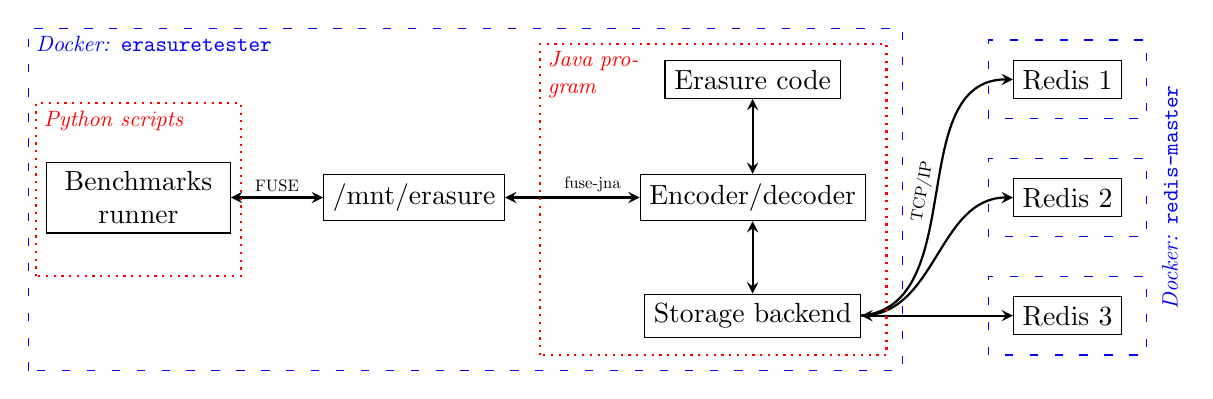
\begin{tikzpicture}
\node[draw, text width=2.1cm, text centered] (bench) at (1.2, 1.5) {Benchmarks runner};
\node[draw] (dir) at (4.7, 1.5) {/mnt/erasure};
\node[draw] (fed) at (9, 1.5) {Encoder/decoder};
\node[draw] (sb) at (9, 0) {Storage backend};
\node[draw] (ec) at (9, 3) {Erasure code};
\node[draw] (r1) at (13, 3) {Redis 1};
\node[draw] (r2) at (13, 1.5) {Redis 2};
\node[draw] (r3) at (13, 0) {Redis 3};

\draw[<->,thick,>=stealth] (bench) -- (dir) node[midway,above,scale=0.6]{FUSE};
\draw[<->,thick,>=stealth] (dir) -- (fed) node[pos=0.65,above,scale=0.6]{fuse-jna};
\draw[<->,thick,>=stealth] (fed) -- (ec);
\draw[<->,thick,>=stealth] (fed) -- (sb);
\draw[->,thick,>=stealth] (sb.east) to[out=5,in=180] node[sloped,midway,scale=0.6,above]{TCP/IP} (r1.west);
\draw[->,thick,>=stealth,out=0,in=180] (sb.east) to[out=0,in=180] (r2.west);
\draw[<->,thick,>=stealth] (sb.east) -- (r3.west);

\draw[loosely dashed,blue] (-0.2,-0.7) rectangle (10.9,3.65);
\draw[loosely dashed,blue] (12,2.5) rectangle (14,3.5);
\draw[loosely dashed,blue] (12,1) rectangle (14,2);
\draw[loosely dashed,blue] (12,-0.5) rectangle (14,0.5);
\draw[dotted,red,thick] (6.3,-0.5) rectangle (10.7,3.45);
\draw[dotted,red,thick] (-0.1,0.5) rectangle (2.5,2.7);

\draw (6.3,3.45) node[below right,red,scale=0.8, text width=1.5cm] {\textit{Java program}};
\draw (-0.1,2.7) node[below right,red,scale=0.8] {\textit{Python scripts}};
\draw (-0.2,3.65) node[below right,blue,scale=0.8] {\textit{Docker:} \texttt{erasuretester}};
\draw (14.3,1.5) node[blue,scale=0.8,rotate=90] {\textit{Docker:} \texttt{redis-master}};
\end{tikzpicture}

	\caption{Graphical representation of the components of the system}
	\label{fig:architecture}
\end{figure}

\section{Software architecture}
\label{subsec:architecture}

This section presents the architecture of the system.
It is graphically summarized in \autoref{fig:architecture}.

The Java program exposes a filesystem by using the \ac{fuse} interface.
When the user runs the program, the filesystem is mounted under a directory of its choice.
The user can then use this directory like it would with any other one.
The tester will intercept system calls by making use of the \textit{fuse-jna} \autocite{fuse-jna} Java library.
Read and write calls will be passed through to the encoder/decoder layer.

The encoder/decoder layer will handle the complicated task of correctly chunking the data.
Its role includes the handling of aligning read and writes operations to the correct boundaries.
Once the data is chunked in blocks of the correct size, it is passed to the erasure coding algorithm, which will add redundancy blocks.
The data and parity blocks will then be passed to the storage backend.

The storage backend is the component that interfaces the block storage primitives of our program to operations on a key-value store.

\subsection{Available implementations}

As stated in \autoref{subsec:architecture}, each component of our tester can have several implementations.
The frontend has one available implementation: a \ac{fuse} filesystem interface backed by \textit{fuse-jna} \autocite{fuse-jna}.
The encoder/decoder layer is not modular because it is sufficient to have one correct way of handling that operation.
There are three erasure coding algorithms bundled with the program.
They come from \autocite{XorbasVLDB}, and were adapted to free them from dependencies on any \textit{Hadoop} component.
A forth algorithm is provided, in the name of the \textit{Null} encoder.
As its name suggests, its \textit{modus operandi} consists in simply forwarding data blocks without any added redundancy.
Our program is compatible with one distributed key-value store: \textit{Redis}.
The compatibility is possible through two libraries: \textit{Redisson} and \textit{Jedis}.
The implementation using \textit{Redisson} is simpler in terms of coding, but is slower.
It is therefore recommended to use the \textit{Jedis} implementation.
For testing purposes, a storage backend using a single Java Map is also available.

\subsection{Blocks storage}

For performance reasons\footnote{This additional component provides a considerable speed-up comprised between $100\times$ and $1000\times$}, there is an additional layer before the storage of blocks in the key-value store.
As the size of each block is 1 byte, performing an operation on the key-value store over the network for each block is very costly.
For this reason, the role of this intermediate layer is to aggregate multiple operations at once.
Instead of storing one block per key in the key-value store, each key stores an aggregation of multiple blocks.
The guarantees offered by the erasure coding process are still kept because one aggregation only stores blocks that belong to the same stripe position.

An \ac{lru} cache optimizes the retrieval of multiple individuals blocks.
This way, when reading a file sequentially, each blocks aggregation is only retrieved once from the key-value store.

\section{Surrounding components}

Running the tester requires multiple independent services.
They need to be launched simultaneously and need to be bootstrapped to work together.
On top of these services, we want to perform measurements on the performance of different erasure codes.
The solution we adopted is the containerization of each service.
The tester along with supporting Python scripts are bundled together in a Docker image.
When an experimenter wants to start the benchmarks with, say, a Redis cluster as storage backend, he only needs to ask Docker Compose to scale the number of running containers.
The supporting Python scripts will configure the Redis cluster and then run the benchmarks and collect the results.

Thanks to the use of Docker Swarm, the setup to run the benchmarks on a local machine or on a cluster of machines is similar.
The system can use any reasonable number of Redis servers.
